%\documentclass[dvipdfmx]{beamer}      % platex の場合
\documentclass[handout]{beamer}        % lualatex の場合
\usepackage{mySld}
\usepackage{multicol}

\begin{document}
\title{基礎コンピュータ工学\\第5章 機械語プログラミング\\(パート10)}
\date{}

\begin{frame}
  \titlepage
  \centerline{\url{https://github.com/tctsigemura/TecTextBook}}
  \vfill
  \centerline{本スライドの入手:
    \raisebox{-7mm}{
\includegraphics[scale=0.3]{../Img/QRs5_A.png}}}
\end{frame}

%==============================================================================
%\begin{frame}
%  \frametitle
%  \tableofcontents
%\end{frame}

\section{論理演算命令}
%==============================================================================
\begin{frame}
  \frametitle{論理演算}
  \emph{「2.8 コンピュータの基本回路」}で学んだ論理演算を再確認.
  \vfill
  \begin{tabular}{l l}
    \emph{論理積(AND)} & \emph{論理和(OR)}      \\
    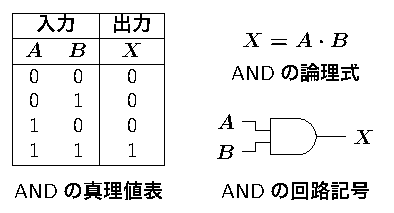
\includegraphics[scale=0.7]{../Tikz/and.pdf}    &
    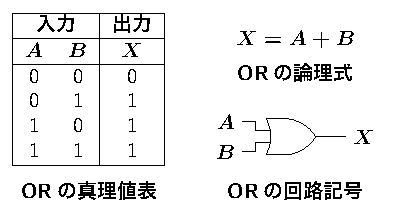
\includegraphics[scale=0.7]{../Tikz/or.pdf}     \\
    \emph{排他的論理和(XOR)} & \emph{否定(NOT)} \\
    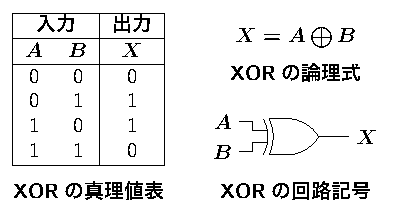
\includegraphics[scale=0.7]{../Tikz/xor.pdf}    &
    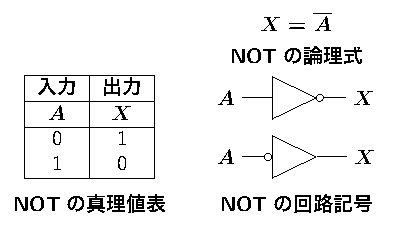
\includegraphics[scale=0.7]{../Tikz/not.pdf}    \\
  \end{tabular}
  \vfill
\end{frame}

%==============================================================================
\begin{frame}
  \frametitle{論理演算命令}
  \emph{論理演算を行うTeCの命令} \\
  8ビットデータを単位に,ビット毎の論理演算を行う. \\
  \centerline{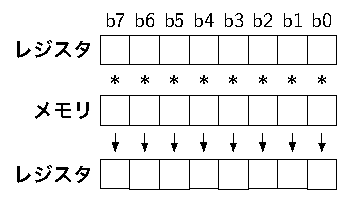
\includegraphics[scale=0.8]{../Tikz/land.pdf}}
  \vfill
  次の3種類がある(NOTはない).
  \begin{itemize}
  \item \emph{論理積(AND)}
  \item \emph{論理和(OR)}
  \item \emph{排他的論理和(XOR)}
  \end{itemize}
  \vfill
\end{frame}

%==============================================================================
\begin{frame}
  \frametitle{AND(Logical AND)命令(論理積)}
  \begin{minipage}{0.48\columnwidth}
  レジスタ値とメモリ値のビット毎の\emph{論理積}を計算し,
  結果をレジスタに格納する.
  \end{minipage}
  \begin{minipage}{0.48\columnwidth}
  \centerline{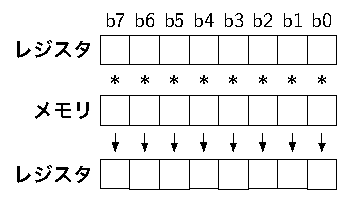
\includegraphics[scale=0.8]{../Tikz/land.pdf}}
  \end{minipage}
  \vfill
  \begin{description}
  \item[Cフラグ] 常に0になる.
  \item[Sフラグ] 結果が負(MSBが1)なら1,それ以外は0になる.
  \item[Zフラグ] 結果がゼロなら1,それ以外は0になる.
    \vfill
  \item[ニーモニック:]\texttt{AND GR,EA}~~~~~~~~~\texttt{(GR ← GR \& [EA])}
    \vfill
  \item[命令フォーマット:] 2バイトの長さを持つ.\\
    {\small\twoByte{$0110_2$}{\GR~\XR}{\A}}
  \end{description}
  \vfill
\end{frame}

%==============================================================================
\begin{frame}
  \begin{description}
  \item[フローチャート:] Javaの演算子を流用する.\\
    \vfill
    \centerline{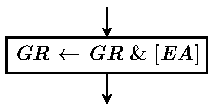
\includegraphics[scale=0.7]{../Tikz/and_chap5.pdf}}
    \vfill
  \item[使用例:]
    A番地のデータとB番地のデータのビット毎の論理積を計算し,
    C番地に格納するプログラムの例を示す.
  \end{description}
  \vfill
  \begin{minipage}{0.58\columnwidth}
    {\ttfamily\small\begin{center}
      \begin{tabular}{|l|l|l|l l|} \hline
        番地 & 機械語 & ラベル & \multicolumn{2}{|c|}{ニーモニック} \\
        \hline
        00 & 10 07 &   & LD   & G0,A \\
        02 & 60 08 &   & AND  & G0,B \\
        04 & 20 09 &   & ST   & G0,C \\
        06 & FF    &   & HALT &      \\
        07 & 63    & A & DC   & 63H  \\
        08 & 0F    & B & DC   & 0FH  \\
        09 & 00    & C & DS   & 1    \\
        \hline
      \end{tabular}
    \end{center}}
  \end{minipage}
  \begin{minipage}{0.38\columnwidth}
    \centerline{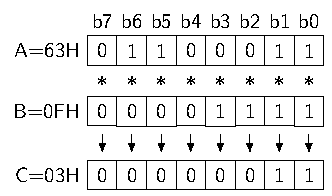
\includegraphics[scale=0.8]{../Tikz/land1.pdf}}
  \end{minipage}
  \vfill
  \vfill
\end{frame}

%==============================================================================
\begin{frame}
  \frametitle{AND命令の応用(1)}
  \emph{特定のビットがゼロか判定する.} \\
  ANDの結果が$00_{16}$かどうかで判断できる.\\
  次は最下位ビット(LSB)を調べる例.\\
  \vfill
  \begin{minipage}{0.48\columnwidth}
    {\small\ttfamily\begin{center}
      \begin{tabular}{|l|l l|l}
        \cline{1-3}
        ラベル & \multicolumn{2}{|c|}{ニーモニック} & \\
        \cline{1-3}
        & ...  &        & \\
        & AND  & G0,ONE & \\
        & JZ   & L1     & \\
        & ...  &        & \\
        L1  & ...  &        & \\
        & ...  &        & \\
        ONE & DC   & 01H    & \\
        \cline{1-3}
      \end{tabular}
    \end{center}}
  \end{minipage}
  \begin{minipage}{0.48\columnwidth}
    \centerline{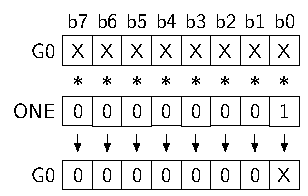
\includegraphics[scale=0.8]{../Tikz/land3.pdf}}
  \end{minipage}
  \vfill
  LSB : Least Significant Bit (最下位ビットのこと, P.10参照)
  \vfill
\end{frame}

%==============================================================================
\begin{frame}
  \frametitle{AND命令の応用(2)}
  \emph{特定のビットを右詰めで取り出す.} \\
  ($b_3$,$b_2$を右詰めで取り出す.)\\
  \begin{minipage}{0.48\columnwidth}
    {\small\ttfamily\begin{center}
      \begin{tabular}{|l|l l|l}
        \cline{1-3}
        ラベル & \multicolumn{2}{|c|}{ニーモニック} & \\
        \cline{1-3}
        & ...  &        & \\
        & AND  & G0,MSK & \\
        & SHRL & G0     & \\
        & SHRL & G0     & \\
        & ...  &        & \\
        MSK & DC   & 0CH    & \\
        \cline{1-3}
      \end{tabular}
    \end{center}}
  \end{minipage}
  \begin{minipage}{0.48\columnwidth}
    \centerline{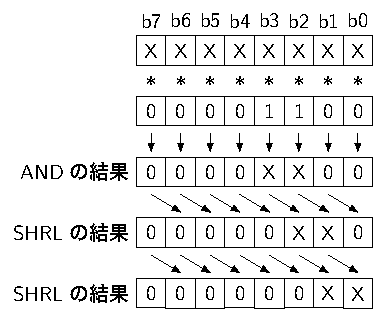
\includegraphics[scale=0.8]{../Tikz/land2.pdf}}
  \end{minipage}
  \vfill
  \vfill
\end{frame}

%==============================================================================
\begin{frame}
  \frametitle{OR(Logical OR)命令(論理和)}
  レジスタ値とメモリ値のビット毎の\emph{論理和}をレジスタに格納する.
  \vfill
  \begin{description}
  \item[Cフラグ] 常に0になる.
  \item[Sフラグ] 結果が負(MSBが1)なら1,それ以外は0になる.
  \item[Zフラグ] 結果がゼロなら1,それ以外は0になる.
    \vfill
  \item[ニーモニック:]\texttt{OR GR,EA}~~~~~~~~~\texttt{(GR ← GR \textbar{} [EA])}
    \vfill
  \item[命令フォーマット:] 2バイトの長さを持つ.\\
    {\small\twoByte{$0111_2$}{\GR~\XR}{\A}}
    \vfill
  \end{description}
  \vfill
  MSB : Most Significant Bit (最上位ビットのこと, P.10参照)
  \vfill
\end{frame}

%==============================================================================
\begin{frame}
  \begin{description}
  \item[フローチャート:] Javaの演算子を流用する.\\
  \vfill
    \centerline{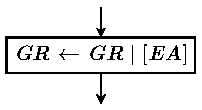
\includegraphics[scale=0.7]{../Tikz/or_chap5.pdf}}
  \vfill
  \item[応用:] G0の上位4ビットを全部1にする.
  \end{description}
  \vfill
  \begin{minipage}{0.48\columnwidth}
    {\ttfamily\small\begin{center}
      \begin{tabular}{|l|l l|l}
        \cline{1-3}
        ラベル & \multicolumn{2}{|c|}{ニーモニック} & \\
        \cline{1-3}
        & ...  &        & \\
        & LD   & G0,DATA& \\
        & OR   & G0,MSK & \\
        & ...  &        & \\
        DATA& DC   & 0AAH    & \\
        MSK & DC   & 0F0H    & \\
        \cline{1-3}
      \end{tabular}
    \end{center}}
  \end{minipage}
  \begin{minipage}{0.48\columnwidth}
    \centerline{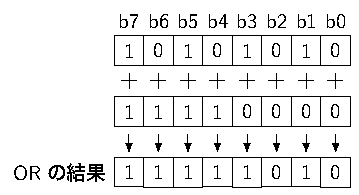
\includegraphics[scale=0.8]{../Tikz/lor.pdf}}
  \end{minipage}
  \vfill
  \emph{16進数の表記:}ラベルと区別が付くように注意!(P.44参照)
  \vfill
\end{frame}

%==============================================================================
\begin{frame}
  \frametitle{XOR(Logical XOR)命令(排他的論理和)}
  レジスタ値とメモリ値のビット毎の\emph{排他的論理和}をレジスタに格納する.
  \vfill
  \begin{description}
  \item[Cフラグ] 常に0になる.
  \item[Sフラグ] 結果が負(MSBが1)なら1,それ以外は0になる.
  \item[Zフラグ] 結果がゼロなら1,それ以外は0になる.
    \vfill
  \item[ニーモニック:]\texttt{XOR GR,EA}~~~~~~~~~\texttt{(GR ← GR \textasciicircum{} [EA])}
    \vfill
  \item[命令フォーマット:] 2バイトの長さを持つ.\\
    {\small\twoByte{$1000_2$}{\GR~\XR}{\A}}
    \vfill
  \end{description}
  \vfill
\end{frame}

%==============================================================================
\begin{frame}
  \begin{description}
  \item[フローチャート:] Javaの演算子を流用する.\\
  \vfill
    \centerline{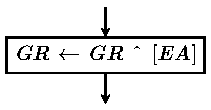
\includegraphics[scale=0.7]{../Tikz/xor_chap5.pdf}}
  \vfill
  \item[応用:] G0上位4ビットの1/0を入れ替える(ビット反転する).
  \end{description}
  \vfill
  \begin{minipage}{0.48\columnwidth}
    {\ttfamily\small\begin{center}
      \begin{tabular}{|l|l l|l}
        \cline{1-3}
        ラベル & \multicolumn{2}{|c|}{ニーモニック} & \\
        \cline{1-3}
        & ...  &        & \\
        & LD   & G0,DATA& \\
        & XOR  & G0,MSK & \\
        & ...  &        & \\
        DATA& DC   & 0AAH    & \\
        MSK & DC   & 0F0H    & \\
        \cline{1-3}
      \end{tabular}
    \end{center}}
  \end{minipage}
  \begin{minipage}{0.48\columnwidth}
    \centerline{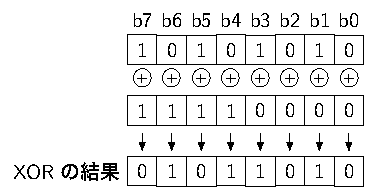
\includegraphics[scale=0.8]{../Tikz/lxor.pdf}}
  \end{minipage}
  \vfill
\end{frame}

%==============================================================================
\begin{frame}
  \frametitle{まとめ}
  \emph{学んだこと}
  \begin{itemize}
  \item ビット毎の論理演算命令
  \item TeCは次の演算命令を持っている.
    \begin{enumerate}
    \item[(1)] \emph{論理積(AND)命令}
    \item[(2)] \emph{論理和(OR)命令}
    \item[(3)] \emph{排他的論理和(XOR)命令}
    \end{enumerate}
  \end{itemize}
  \vfill
  \emph{演習}
  \begin{itemize}
  \item TeCにはNOT命令が無い.\\
    NOT命令があったとすると,どんな計算をする命令になるか?
  \item NOT命令の代用となる命令を考えなさい.
  \item 値が奇数か偶数か判定する方法を考えなさい.
  \item 8で割った余りを計算する方法を考えなさい.
  \end{itemize}
  \vfill
\end{frame}

\end{document}
